% Required packages: texlive-bibtex-extra texlive-publishers

\documentclass[10pt, oneside, letterpaper]{article}
\usepackage[utf8]{inputenc}

\usepackage{authblk}
	\setcounter{Maxaffil}{0}
	\renewcommand\Affilfont{\itshape\small}
\usepackage[justification=centering]{caption}
\usepackage{float}
\usepackage[margin=1.5in]{geometry}
\usepackage{graphicx}
	\graphicspath{ {img/} }
\usepackage[colorlinks=true, linkcolor=blue, urlcolor=blue, citecolor=blue]{hyperref}
\usepackage{indentfirst}
\usepackage{multicol}
\usepackage{ragged2e}  % For ragged right bibliography
\usepackage{verbatim}

\title{\textbf{Technological Enhancement:\\An Imminent Social Recategorization of Beyond-Human Abilities}}
\author{Jeffrey Leung}
\affil{Simon Fraser University}
\date{December 2, 2019}

\begin{document}

	\maketitle

	\begin{abstract}
		This paper is an assignment for SEE 101W: Process, Form and Convention in Professional Genres. Technological aspirations and societal expectations will conflict in the near future. Bionic technology is designed to replace and improve upon existing human body abilities, and this technology is advancing rapidly. Society is built upon the expectations of naturally limited human abilities in areas such as security, education, and athletics. The following question is raised: if a person is augmented beyond natural human abilities by bionic enhancements, should they be categorized alongside other naturally capable humans in society, or re-categorized into a new distinct area of comparison? This paper tackles this imminent humanistic and ethical dilemma created by rapidly improving technology. We conclude that a re-categorization is necessary, but the process need not be an ostracism but can instead be a celebration of evolved ability.
	\end{abstract}

	\begin{multicols}{2}

	\section{Introduction}

	The capabilities of technology in everyday life has advanced to levels matching science-fiction imagination half a century ago. Our devices are capable of interplanetary spaceflight, destruction of immense swathes of lands, and navigation of dangerous rescue situations, but the most impactful developments to us personally are the technologies we utilize to improve our lives and abilities. In the last decade, major strides in research have been made towards the creation of powerful prostheses and exoskeletons \cite{Benabid2019}. Already, cybernetic prostheses are capable of enhancing our abilities beyond standard human levels. This undermines the standard societal expectations of human limitations in areas such as athletics, education, and security. Consequently, the question arises: if a person is augmented beyond natural human abilities by bionic enhancements, should they be categorized alongside other naturally capable humans in society, or re-categorized into a new distinct area of comparison? Can a human with the same cognitive abilities but superhuman physical abilities still be justly compared with any other normal human? Societal reclassification of technologically augmented humans must occur in the near future due to the nature of competition in athletics and the progress of learning in standardized education.

	\section{Precedence for a New Ostracism}

	To understand the societal underpinnings of this issue, the nature of technological augmentation and social in-grouping must be analyzed. For clarity throughout this paper, we will refer to ``augmented humans'' as those who are cybernetically and technologically enhanced through limb replacement, neural implants, or other such biological enhancement technology which allows them to possess superhuman abilities and exceed natural limitations. Inversely, we will refer to ``natural humans'' as those who do not possess technological enhancements to their body and are only capable of biologically limited human abilities.

	\subsection{Beyond Human Abilities}

	The current capabilities of technological enhancement are already sufficiently advanced to improve and exceed a standard quality of human life. Prominent researchers such as Hugh Herr, a double amputee who became a researcher after losing both legs, work in the fields of biology, mechanics, electronics, and control to create complex bionics capable of mimicking human abilities \cite{Isobarista2018}. Benabid et al. \cite{Benabid2019} describe an exoskeleton successfully designed to provide a tetraplegic patient (paralyzed in all 4 limbs) with a full range of motion which is controlled via a neural implant on the surface of the brain. Recent developments of exoskeleton robots which augment soldiers in moving large amounts of weight and carrying out teleoperations are studied by Gopura et al. \cite{Gopura2016} (see Figure \ref{fig:uprise-exoskeleton} for an exoskeleton).

	\begin{figure}[H]
		\centering
		
\includegraphics[width=\linewidth]{uprise-exoskeleton}
		\caption{A soldier utilizes the UPRISE Exoskeleton to reduce carried weight by up to 80\%. Adapted from \protect\cite{Army2019}}
		\label{fig:uprise-exoskeleton}
	\end{figure}

	\subsection{In Popular Culture}

	Science fiction and popular culture often toy with tantalizing ideas of incredible technology capable of creating a hostile divide. For example, robots constructed with advanced technology are imagined to be near indistinguishable from humans and capable of supreme emotion and cognition such as the replicants from Blade Runner or the hosts from Westworld. Another common theme is the vast amounts of technological enhancements to a human body to reach extreme levels of perception and combat such as the characters from the video game Deus Ex: Human Revolution (see Figure \ref{fig:deus-ex} for an illustration of the main character).

	\begin{figure}[H]
		\centering
		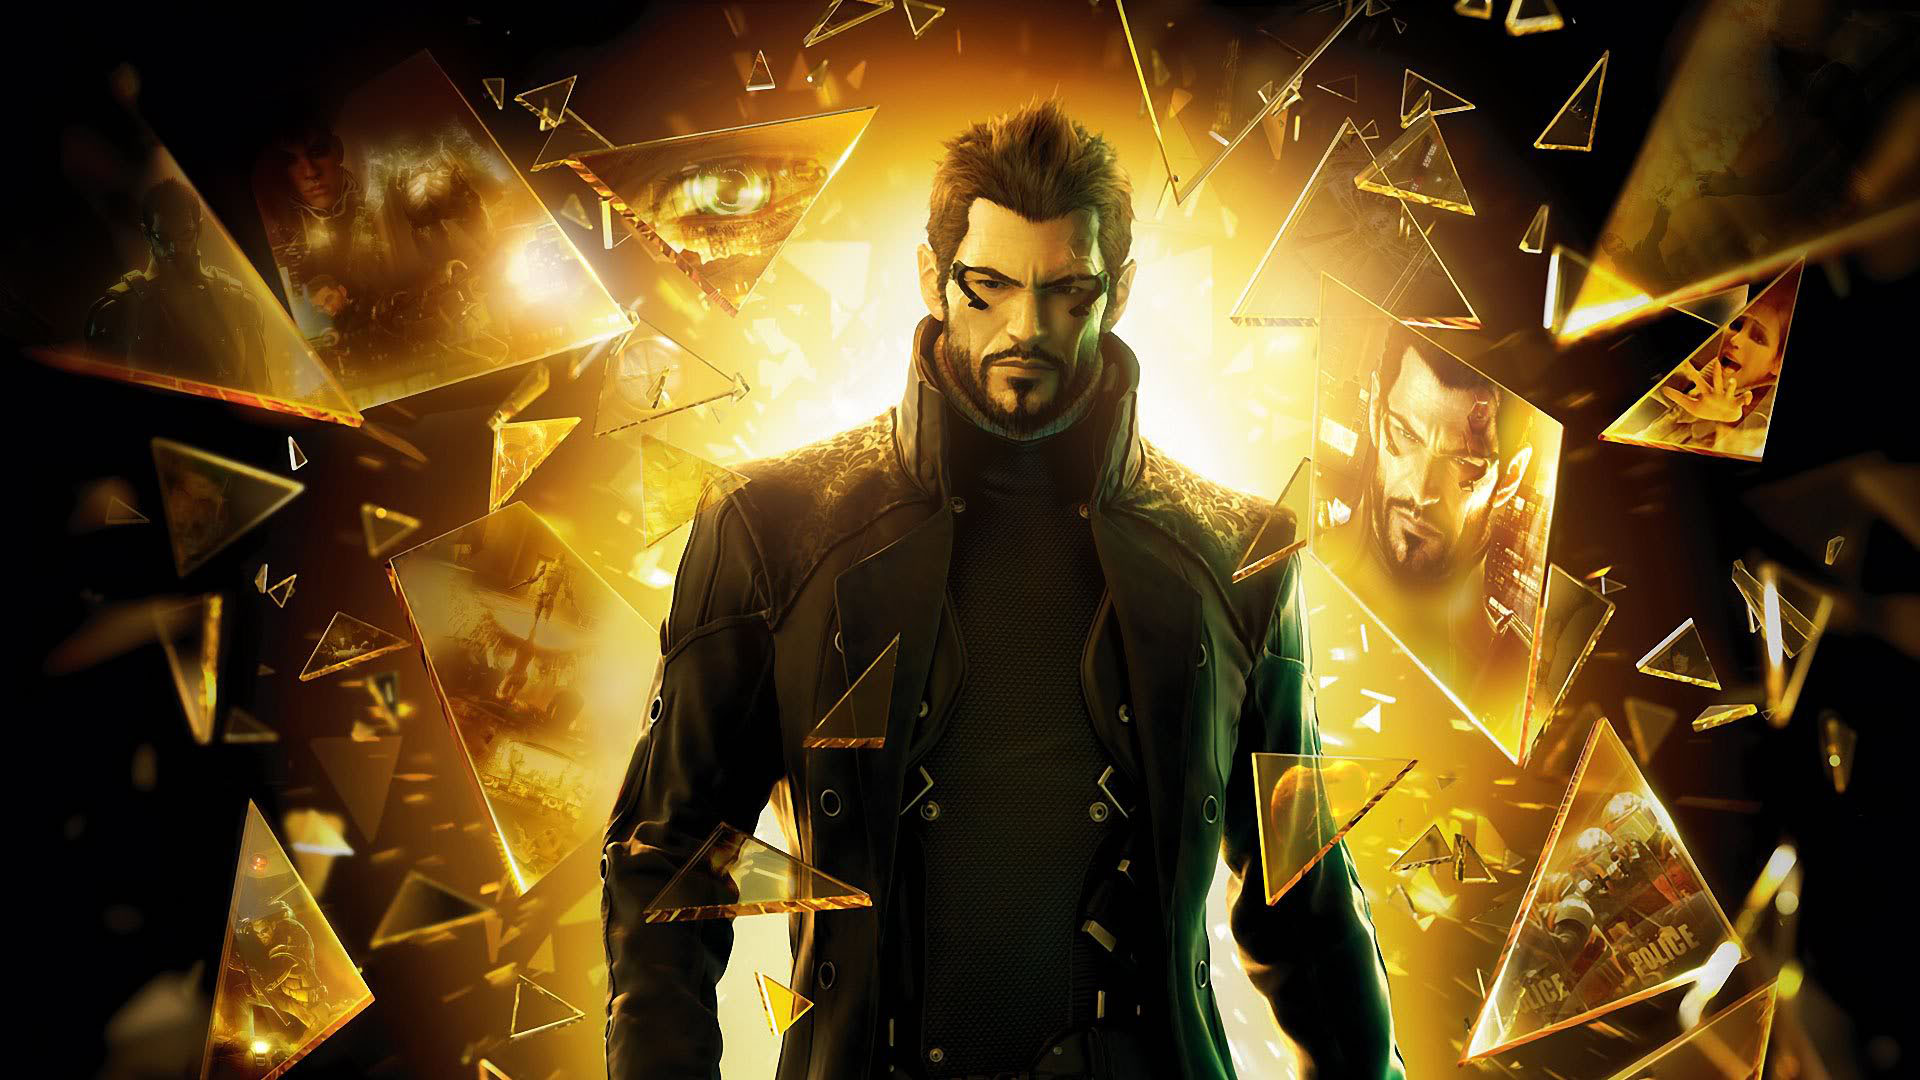
\includegraphics[width=\linewidth]{deus-ex}
		\caption{The heavily augmented Adam Jensen in Deus Ex. Adapted from \protect\cite{Lieu2018}}
		\label{fig:deus-ex}
	\end{figure}

	In her scientific article More Than Merely Human: How Science Fiction Pop-Culture Influences Our Desires for the Cybernetic, Gibson \cite{Gibson2017} analyzes the imminent possibility of near-human cyborgs and the consequences of augmentation which replaces most of our humanity. In short, she describes the ``search for authenticity—for that which is genetically, biologically, non-mechanically human.'' Gibson also analyzes the novel Do Androids Dream of Electric Sheep? for its thematic search for authenticity which creates the question ``What constitutes `us' and how does it differ from `them'?'' The game Detroit also has a character who is incapable of independent thought and emotion and Gibson describes how this separates the robot from the human identity. These are culturally relevant perspectives, and the marked differences between natural humans and enhanced humans convey a clear message: They are very much like us but they are not the same.

	\section{The Physical Dimension: Cybernetics in Athletics}

	\subsection{The Pistorius Controversy}

	For years, cybernetic enhancement of human ability has been disrupting standardized competitions. Nowhere is this more starkly evident than in the field of athletics where people hone competitive skill and physical power over years of tireless practice. In 2008, Oscar Pistorius, a double amputee runner, was banned from competing in the 2012 Olympic Games in London. This was due to his light prosthetic ``spring'' legs for running, which were marketed to utilize 25\% less energy than the energy used by natural runners \cite{Evelith2012}. See Figure \ref{fig:pistorius} for an image of Pistorius sprinting with his prosthetic legs.

	\begin{figure}[H]
		\centering
		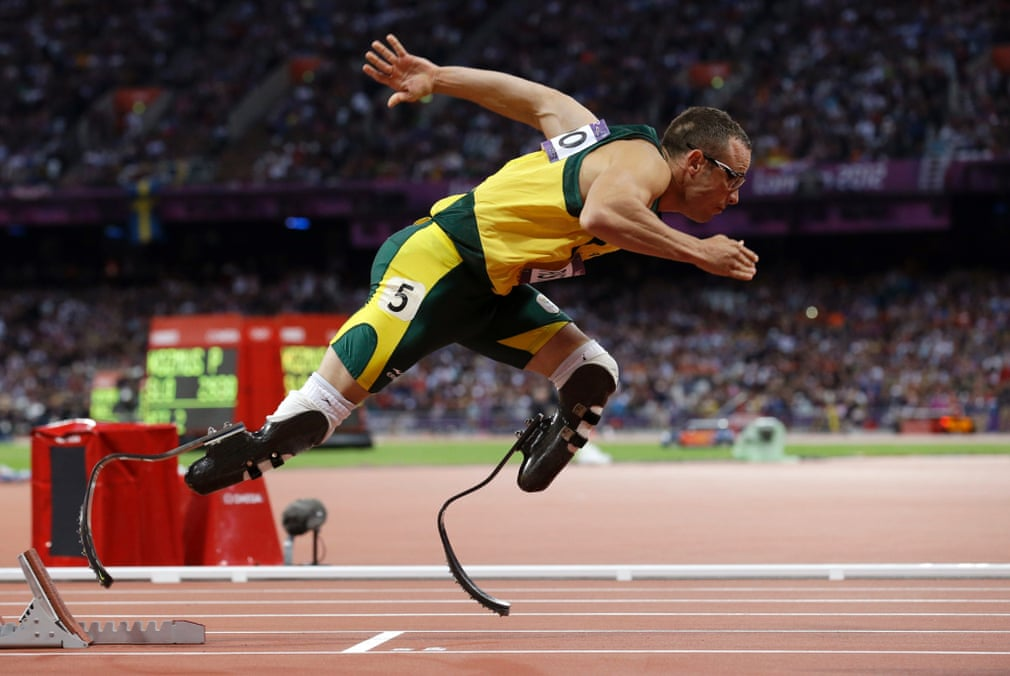
\includegraphics[width=\linewidth]{pistorius}
		\caption{Oscar Pistorius competes in the men's 400-meter athletics semi-final. Adapted from \protect\cite{Niedringhaus2012}}
		\label{fig:pistorius}
	\end{figure}

	A scientific study by prominent biophysicists commissioned to determine the exact differences found that he consistently had 25\% less aerial and swing times for his legs than other runners, concluding he was ``physiologically similar but mechanically dissimilar'' to a runner with normal legs \cite{Weyand2009}. Though Pistorius was reluctantly allowed to compete, there is still controversy about whether or not this was fair.

	\subsection{Re-categorization}

	There is already precedent that augmented humans may be judged to be unfair competition for those who possess natural human abilities. As technological enhancements improve, the gap between peak abilities of natural humans and enhanced humans will continue to widen enough that it can no longer be ignored. At this point, a new category should be created across the field of athletics to judge those who are augmented, in the same way that the Paralympics create a category for athletes with lesser capabilities than normally capable humans.

	\subsection{The Counterargument}

	An argument might be that the development of technology should be limited to the peak ability of humans, so as not to create inferiority and superiority. This difference would be compounded by social factors such as high costs, leading to a chasm between the haves and have-nots. However, a counterargument is that improving human ability is already impacted by the wealth gap as those who are more affluent have greater time, resources, and connections to improve their well-being. To counter the base argument, methods such as medicine are ethical even when they improve human ability beyond natural limitations. if the problem of equitable access can be solved, then it will be illogical to withhold such technologies. These technologies can reach beyond physical capabilities, and can even enhance cognitive abilities.

	\section{The Mental Dimension: Technological Enhancement in Education}

	\subsection{Neural Enhancement}

	Standardized education and testing have always relied on the limitations of natural ability. In most scenarios of evaluation, calculators are banned, notes are disallowed, and phones are prohibited. With the advent of technology that improves educational and developmental ability, artificially-imposed limitations are weakening. Marchesi and Riccò \cite{Marchesi2013} introduce a new e-learning system that utilizes a direct brain-computer interface to provide a user with neurofeedback about their current learning ability, which can in turn be used to customize educational content to a student's needs. In addition, Clites et al. \cite{Clites2018} study how neural interfaces can be designed to provide awareness of the position and speed of bionic limbs to the brain. It is not difficult to see how neural interfaces can understand brain signals and designed to provide calculated feedback to the user.

	If it becomes possible for humans to achieve greater cognitive capability using a neurally implanted device, then large swaths of standardized education could become invalidated due to the abilities of some people to utilize embedded non-removable systems which process information more effectively. At this point, the categorization due to compared ability would need to be re-evaluated and redesigned to allow for significantly greater cognitive potential, without invalidating those with natural limitations.

	\subsection{The Counterargument}

	An argument against this would be that education is focused not on human limitations but rather on improving the cognitive abilities along guide rails designed to evaluate the progress of these abilities. This is only partially valid, as the education system would still need to be revised to encourage growth and learning while reducing the weight of performance evaluation based on comparisons with other students in the same year and class. Grade results are overutilized in society as a measure of potential and ability - a flaw inherent to the system which requires improvement. Education is not ready for the capabilities of cybernetic enhancements, but it could potentially be through revising the standardized evaluation environment.

	\section{Conclusion}

	The answer to the proposed question of categorizing enhanced humans is nuanced, but the drive to develop the technological capability to create superhuman ability is strong. Technology is improving at a rapid pace and will only continue advancing. Society will soon be confronted with the choice of implanting superhuman abilities as well as the consequences that will follow to our current systems built upon natural human ability, including athletic competitions and educational development. At all costs, society must work to avoid ostracism and the process of ingrouping and outgrouping. This must be done by creating a new common ideal of human ability to strive towards, rather than aiming to defy standards and safety through creating disruptive technology.

	\end{multicols}

	{\RaggedRight
		\bibliographystyle{IEEEtran}
		\bibliography{technological-enhancement-an-imminent-social-recategorization}
	}

\end{document}
